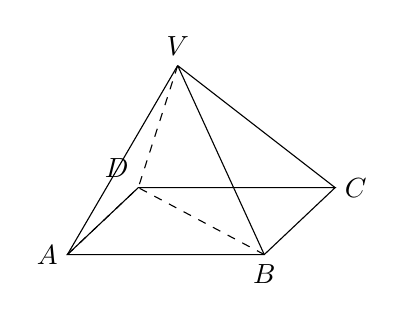
\begin{tikzpicture}[scale=1.0]
  \coordinate (V) at (0.1,2.4);
  \coordinate (A) at (-1.3,0);
  \coordinate (B) at (1.2,0);
  \coordinate (C) at (2.1,0.85);
  \coordinate (D) at (-0.4,0.85);
  \draw (V) -- (A) (V) -- (B) (V) -- (C);
  \draw (A) -- (B) -- (C) -- (D) -- cycle;
  \draw[dashed] (V) -- (D);
  \draw[dashed] (A) -- (D);
  \draw[dashed] (B) -- (D);
  \node[above] at (V) {$V$};
  \node[left] at (A) {$A$};
  \node[below] at (B) {$B$};
  \node[right] at (C) {$C$};
  \node[above left] at (D) {$D$};
\end{tikzpicture}
